%%%%%%%%%%%%%%%%%%%%%%%%%%%%%%%%%%%%%%%%%%%%%%%%%%%%%%%%%%%%%%%%%%%%%%%%
\chapter{Implementation Details}
%%%%%%%%%%%%%%%%%%%%%%%%%%%%%%%%%%%%%%%%%%%%%%%%%%%%%%%%%%%%%%%%%%%%%%%%

\section{Reference Implementation}
\label{sec:reference-implementation}

This section will present a quick overview of relevant parts of the reference implementation.

The reference implementation is hosted as a public GitHub repository \cite{github:2017:lyra}. There are several projects in the same repository (both Lyra2 and Lyra, as well as documentation). The Lyra2 directory of the master branch contains the latest version of the code and documentation. In particular, \path{Lyra2/src} is the root directory for code, \path{Lyra2/src/bench} contains benchmarking shell scripts, \path{Lyra2/src/cuda} contains code that studies how Lyra2 withstands GPU-based attacks, \path{Lyra2/src/sse} contains an sse-optimized implementation. Finally, the \path{Lyra2/src} contains the reference implementation in C99 and is the primary focus of this work.

The original public repository \cite{github:2017:lyra} was forked to \cite{github:2017:lyra-copy} and the following modifications were made. The reference implementation uses \verb|make| as its build system and the \path{Lyra2/src/makefile} provides clear compilation instructions. However, only one version of Lyra2 could conveniently be compiled and the provided test vectors are hard-coded into the program. So, the following functionality was added for a more conventient comparison of the reference implementation to its ported Java version:

\begin{itemize}
    \item Compile multiple versions of Lyra2 which could be used simultaneously.
    \item Compute and store hash values of some test inputs for each version of Lyra2.
  \end{itemize}

This functionality can be found on the \verb|harness| branch of the forked repository \cite{github:2017:lyra-copy} and a pull request \cite{github:2017:lyra-pr} to the original public repository. It is a Python 3 script \verb|Lyra2/tests/harness.py| which can be configured both on the command line and the \verb|Lyra2/tests/harness.yml| configuration file. The \verb|Lyra2/tests/harness.py compile| compiles several Lyra2 reference implementations and the \verb|Lyra2/tests/harness.py compute| runs those implementations on a series of test vectors and records the resulting hash values.

\section{Java Implementation}

It is well known that C is primarily a function-based language. At the same time Java is a lot more object-oriented. Therefore, the C functions from the reference implementation need to be translated into (abstract) classes and interfaces in Java. An additional challenge is the fact that the reference implementation uses conditional compilation, so a function with the same name actually contains different code depending on the instructions received by the compiler.

The architecture of the Java project underwent iterative improvements and a reasonably accurate UML diagram of the final version can be seen in figure \ref{fig:uml}.


\begin{figure}
\begin{tikzpicture}
    \begin{umlpackage}{lyra2}
        \umlclass{Main}{}{
            \umlstatic{
                + main(argv: String[]): void
            }
        }

        \umlclass[right=1cm of Main]{mem}{}{
            \umlstatic{
                + copy(dst: byte[], offset: int, src: int): void
            } \\
            \umlstatic{
                + flip(x: long): long
            }
        }

        \umlclass[below=0.5cm of Main]{echo}{}{
            \umlstatic{
                + bytes(bytes: byte[], n: int, m: int, s: int): void
            } \\
            \umlstatic{
                + bytes(bytes: byte[], n: int): void
            } \\
            \umlstatic{
                + bytes(longs: long[], n: int, m: int, s: int): void
            } \\
            \umlstatic{
                + bytes(longs: long[], n: int): void
            } \\
            \umlstatic{
                + params(params: LyraParams): void
            }
        }

        \umlclass[right=1cm of echo]{pack}{}{
            \umlstatic{
                + bytes(x: long): byte[]
            } \\
            \umlstatic{
                + bytes(longs: long[]): byte[]
            } \\
            \umlstatic{
                + longs(bytes: byte[]): longs[]
            } \\
            \umlstatic{
                + bytes(strings: String[]): byte[]
            }
        }


        \umlclass[below right=0.5cm and -6cm of echo]{Lyra2}{}
        {
            \umlstatic{
                + phs(hash: byte[], pass: byte[], salt: byte[], params: LyraParams): void
            } \\
            \umlstatic{
                + hash(hash: byte[], pass: byte[], salt: byte[], params: LyraParams): void
            }
        }

        \umlclass[below=0.5cm of Lyra2]{Sponge}{
            + state: long[]
        }{
            + absorb(src: long[], len: int, offset: int): void \\
            + squeeze(dst: byte[], len: int): void \\
            + sponge\_lyra(rounds: int): void \\
            \umlstatic{
                + rotr64(word: long, b: int): void
            } \\
            \umlstatic{
                + rotl64(word: long, b: int): void
            } \\
            \umlvirt{
                + G(a: int, b: int, c: int, d: int): void
            } \\
            + reduced\_squeeze\_row0(dst: long[], offset: int): void \\
            + reduced\_duplex\_row1\_and\_row2(dst: long[], offset1: int, offset2: int): void \\
            + reduced\_duplex\_row\_filling(dst: long[], offset0: int, offset1: int, offset2: int, offset3: int): void \\
            + reduced\_duplex\_row\_wandering(dst: long[], offset0: int, offset1: int, offset2: int, offset3: int): void
        }

        \umlclass[below left=0.5cm and -6cm of Sponge]{SpongeBlake2b}{}{
            + G(a: int, b: int, c: int, d: int): void
        }

        \umlclass[below left=0.5cm and -15cm of Sponge]{SpongeBlamka}{}{
            + G(a: int, b: int, c: int, d: int): void
        }

        \umlclass[below=3cm of Sponge]{SpongeHalfBlamka}{}{
            + G(a: int, b: int, c: int, d: int): void
        }

        \umlHVinherit{SpongeBlake2b}{Sponge}
        \umlHVinherit{SpongeBlamka}{Sponge}
        \umlHVinherit{SpongeHalfBlamka}{Sponge}
      \end{umlpackage}
  \end{tikzpicture}
  \caption{Approximate class diagram for \texttt{com.github.all3fox.lyra2} package}
  \label{fig:uml}
  \end{figure}

The \texttt{Main} class is the entry point of the project. An implementational detail that is not shown in figure \ref{fig:uml} is that the \texttt{Main} class relies on a 3\textsuperscript{rd} party command line library \verb|picocli| \cite{web:2017:picocli} that parses input parameters (like the password, the salt, etc.) and constructs an instance of the \texttt{LyraParams} class. That class is also not shown in the figure, it just stores the parametrs and constants relevant to Lyra2's operation. Finally, the \texttt{echo} class is a collection of methods for pretty-printing different types of arrays as a table of bytes to the console.

The \texttt{mem} and \texttt{pack} classes are responsible for memory manipulations. In particular, the \texttt{mem} class deals with the little- and big-endian discrepancies between the C and Java ecosystems on the \texttt{x86\_64} architecture. The \texttt{C99} is little-endian, which results in bytes being reversed when written to memory, as shown in figure \ref{fig:little-endian}. At the same time the Java virtual machine is big-endian. The \texttt{pack} class provides methods that allow to emulate the recasting of the \texttt{void*} pointer to other kinds of pointers (for instance, the \texttt{uint64\_t*} or the \texttt{char*} pointers).

\begin{figure}
    \centering
    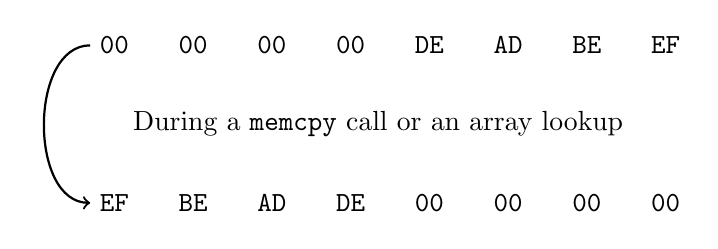
\begin{tikzpicture}
        \node (0)              {\texttt{00}};
        \node (1) [right of=0] {\texttt{00}};
        \node (2) [right of=1] {\texttt{00}};
        \node (3) [right of=2] {\texttt{00}};
        \node (4) [right of=3] {\texttt{DE}};
        \node (5) [right of=4] {\texttt{AD}};
        \node (6) [right of=5] {\texttt{BE}};
        \node (7) [right of=6] {\texttt{EF}};

        \node (H0) [below of=0] {};

        \node (A) [below of=H0]  {\texttt{EF}};
        \node (B) [right of=A] {\texttt{BE}};
        \node (C) [right of=B] {\texttt{AD}};
        \node (D) [right of=C] {\texttt{DE}};
        \node (E) [right of=D] {\texttt{00}};
        \node (F) [right of=E] {\texttt{00}};
        \node (G) [right of=F] {\texttt{00}};
        \node (H) [right of=G] {\texttt{00}};

        \draw [thick,out=180,in=180,->] (0) to node [right=1cm] {During a \texttt{memcpy} call or an array lookup} (A);
      \end{tikzpicture}
    \caption{The byte swap on a little-endian platform (i.e. C99 on \texttt{x86\_64})}
    \label{fig:little-endian}
  \end{figure}

The \texttt{Lyra2} class contains the main logic of the single-threaded Lyra2 instance. The functionality related to the sponge construction is captured by the \texttt{Sponge} \emph{abstract} class. Its subclasses \texttt{SpongeBlake2b}, \texttt{SpongeBlamka} and \texttt{SpongeHalfBlamka} hold the specifics of the underlying fixed-width permutation \(f\).

An insteresting detail is that the Sponge class in the Java project makes use of both left- and right bit rotations, done by the \texttt{rotl64} and \texttt{rotr64} methods respectively. The original Lyra2 reference implementation requires just one direction for rotations. Both types of rotations are helpful in the ported Java project because they allow to avoid a number of byte rotations related to endianness. For an example of this,  refer to figure \ref{fig:sponge-blake2b}. It shows the \texttt{SpongeBlake2b} implementation, where lines \(5, 8\), and \(11\) use a left rotation. This happens because the rotations there involve a whole number of bytes and there is no \texttt{mem.flip} call which performs an endianness-related rotation. On the contrary, line \(16\) expects a none-whole byte rotation (i.e. one bit rotation) which does not allow to repeat the same trick.


\begin{figure}
\small
\begin{minted}[linenos]{java}
    public class SpongeBlake2b extends Sponge {
        @Override
        public void G(final int a, final int b, final int c, final int d) {
            state[a] = mem.flip(mem.flip(state[a]) + mem.flip(state[b]));
            state[d] = rotl64(state[d] ^ state[a], 32);

            state[c] = mem.flip(mem.flip(state[c]) + mem.flip(state[d]));
            state[b] = rotl64(state[b] ^ state[c], 24);

            state[a] = mem.flip(mem.flip(state[a]) + mem.flip(state[b]));
            state[d] = rotl64(state[d] ^ state[a], 16);

            state[c] = mem.flip(mem.flip(state[c]) + mem.flip(state[d]));
            // Cannot use the left rotation trick here: 63 % 8 != 0, so
            // individual bytes do not stay the same, they change too.
            state[b] = mem.flip(rotr64(mem.flip(state[b] ^ state[c]), 63));
        }
    }
\end{minted}
\normalsize
\caption{Blake2b as instance of the Sponge class, illustrating optimized rotations}
\label{fig:sponge-blake2b}
\end{figure}
